\section{Durchführung}
\label{sec:Durchführung}
\subsection{Versuchsaufbau}
Zentral in diesem Versuch ist die Röntgenstrahlung welche durch eine Öffnung an der Mantelfläche eines Zylinders, in dessen Mitte das Probenstäbchen sitzt, auf die Probe gestrahlt wird und dabei gestreut wird. 
Die Innenseite des Mantels des Metallzylinders ist vollständig mit einem Film bedeckt.
Die Achse des Probenstäbchens steht senkrecht auf den beiden Deckeln des Zylinders. Eine schematische Skizze das Aufbaus ist in \ref{fig:Aufbau} gegeben.
\begin{figure}
	\centering
	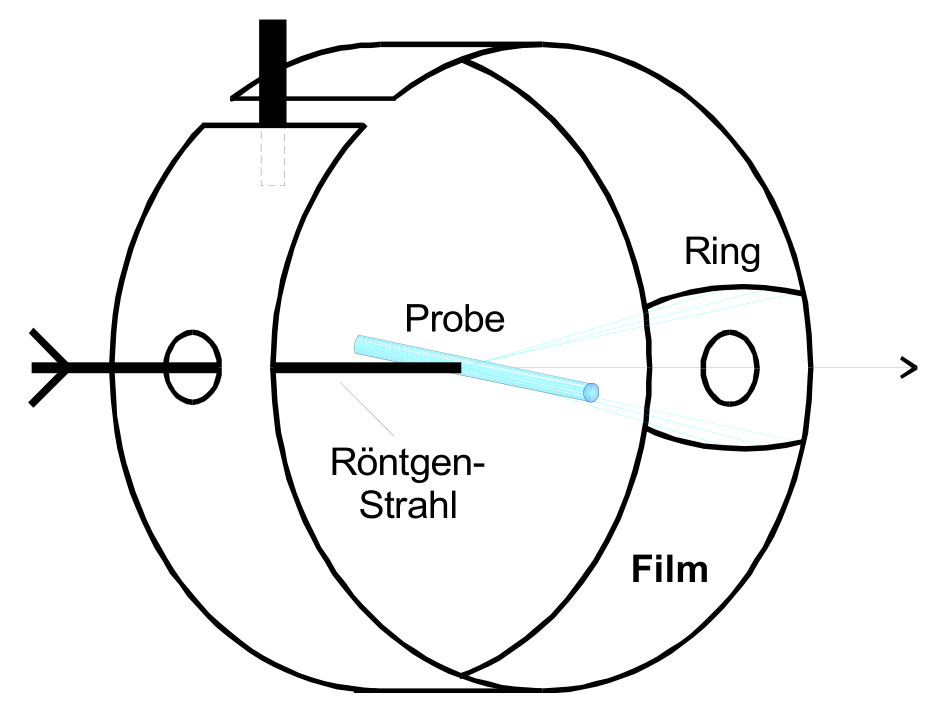
\includegraphics[width = \textwidth]{Abbildungen/Aufbau.png}
	\caption{Der Aufbau zeigt den Film in der Kamera, sowie die Probe und den EIngang der Röntgenstrahlung und ein mögliches Beugungsmuster an der rechten Seite des Films in der Skizze \cite{Anleitung}. }
	\label{fig:Aufbau}
\end{figure}  
Der ganze Zylinder ist bis auf die Öffnung für die Röntgenstrahlung lichtdicht verschlossen.
Außen am Zylinder, an der Fassung des Probenstäbchens ist ein Motor angebracht, mit dem die Probe gedreht wird.
Der Zylinder ist sozusagen das Kameragehäuse und wird im weiteren Verlauf als Kamera bezeichnet. 
Die Fassung selber ist so justierbar, dass das Probenstäbchens möglichst mittig zur Öffnung des Röngenstrahls steht.\\
Die Röntgenstrahlen werden durch eine Röntgenröhre erzeugt, welche eine Kupferanode besitzt.
Die Beschleunigungsspannung ist dabei deutlich gräßer, als die Kathodenspannung und beträgt \SI{40}{\kV}. 
Dabei werden die charakterisctischen Emissionslinien K$_{\alpha 1}$, K$_{\alpha 2}$ und K$_\beta$ erzeugt. 
Die K$_\beta$-Linie ist ncht relevant.  
Sie wird durch Nickel absorbiert.

\subsection{Preparation der Probe}
Das Probenstäbchen ist ein einfaches Glasstäbchen, welches mit dem zu untersuchenden Stoff benetzt wird.
Dazu wird das Probenstäbchen in Vaseline eingetacht und dann in dem Probenmaterial gedreht, sodass eine dünne Schicht auf der Oberfläche des Stäbchens entsteht. 
Die Stäbchen messen alle ungefähr 0.8 \si{\milli \meter} im Durchmesser.
Dann muss das präparierte Probenstäbchen in einen passenden Halter gesteckt und dann in die Kamera eingebaut werden.

\subsection{Entwicklung der Filme}
Der Film wird dann in einer Dunkelkammer entwickelt. 
Das wird in drei Stufen ausgeführt, wobei zwischen den drei Phasen der Film in einem Wasserbad durch Schwenken gereiningt wird.\\
In der ersten Phase wird der Film auf eine Spule gewickelt und in ein Gefäß mit Entwicklungsflüssigkeit 15 Minuten lang geschwenkt.
Die zweite Phase nutzt einen UNterbrecherbad, in der der Film ca. 1 Minute lang getacht wird. \\
Zum Schluss wird der Film dann wieder, in einem Gefäß mit einer Fixierflüssigkeit, 5 Minuten lang geschwenkt.
Danach trocknet der Film 30 Minuten in einer Heißluftkammer.
 







